\vspace*{\subsecspace}
%\section{Experimental Evaluation}
%\section{Model Testing and Validation}
%\section{Testing and Evaluation of Model-Informed Policies}
\section{Model and Policy Evaluation}
\label{sec:eval}

%%\vspace*{\subsecspace}
%\section{SciSpot Design and Implementation}
\subsection{Details of the Experimental Framework used for Evaluation}
%\section{Model-Informed Policy Implementation}
\label{sec:impl}


\sysname is a general-purpose software framework for running scientific computing applications on low-cost transient cloud servers.
It incorporates policies and mechanisms for generating, deploying, orchestrating, and monitoring bags of jobs on cloud servers.
Specifically, it runs a bag of jobs defined by these parameters:
\begin{lstlisting}[basicstyle=\sffamily, frame=single, columns=fullflexible, escapeinside={(*}{*)}]
  Bag of job = {(*$\mathcal{A}$*): Application to execute,
  (*$n$*): Number of jobs,
  (*$m$*): Minimum number of jobs to finish,
  (*$\pi$*): Generator function for job parameters,
  (*$\mathcal{R}$*): Computing resources per job}
\end{lstlisting}


%Additionally, ease-of-use is one of \sysname's primary design goals, and we specifically incorporate

%it is suitable for running a large variety of applications.
\sysname seeks to minimize the cost and running time of bags of jobs of scientific computing applications.
\sysname's cost and time minimizing policies for running bags of jobs are based on empirical and analytical models of the cost and preemption dynamics of  transient cloud servers, which we present in the next section. 

\sysname is designed as a framework that increases the usability and viability of transient cloud servers for scientific computing applications, and provides a simple user interface to allow users to deploy their applications with minimum workflow changes. 
Most scientific computing applications are deployed on HPC clusters that have a batch scheduler such as Slurm~\cite{slurm} or Torque~\cite{torque}, and \sysname integrates with these schedulers (e.g., Slurm) to provide the same interface to applications. 
As shown in Figure~\ref{fig:arch},
\sysname creates and manages clusters of transient cloud servers, manages all aspects of the VM lifecycle and costs, and implements the various policies described in the rest of this section. 

\begin{figure}[t]
  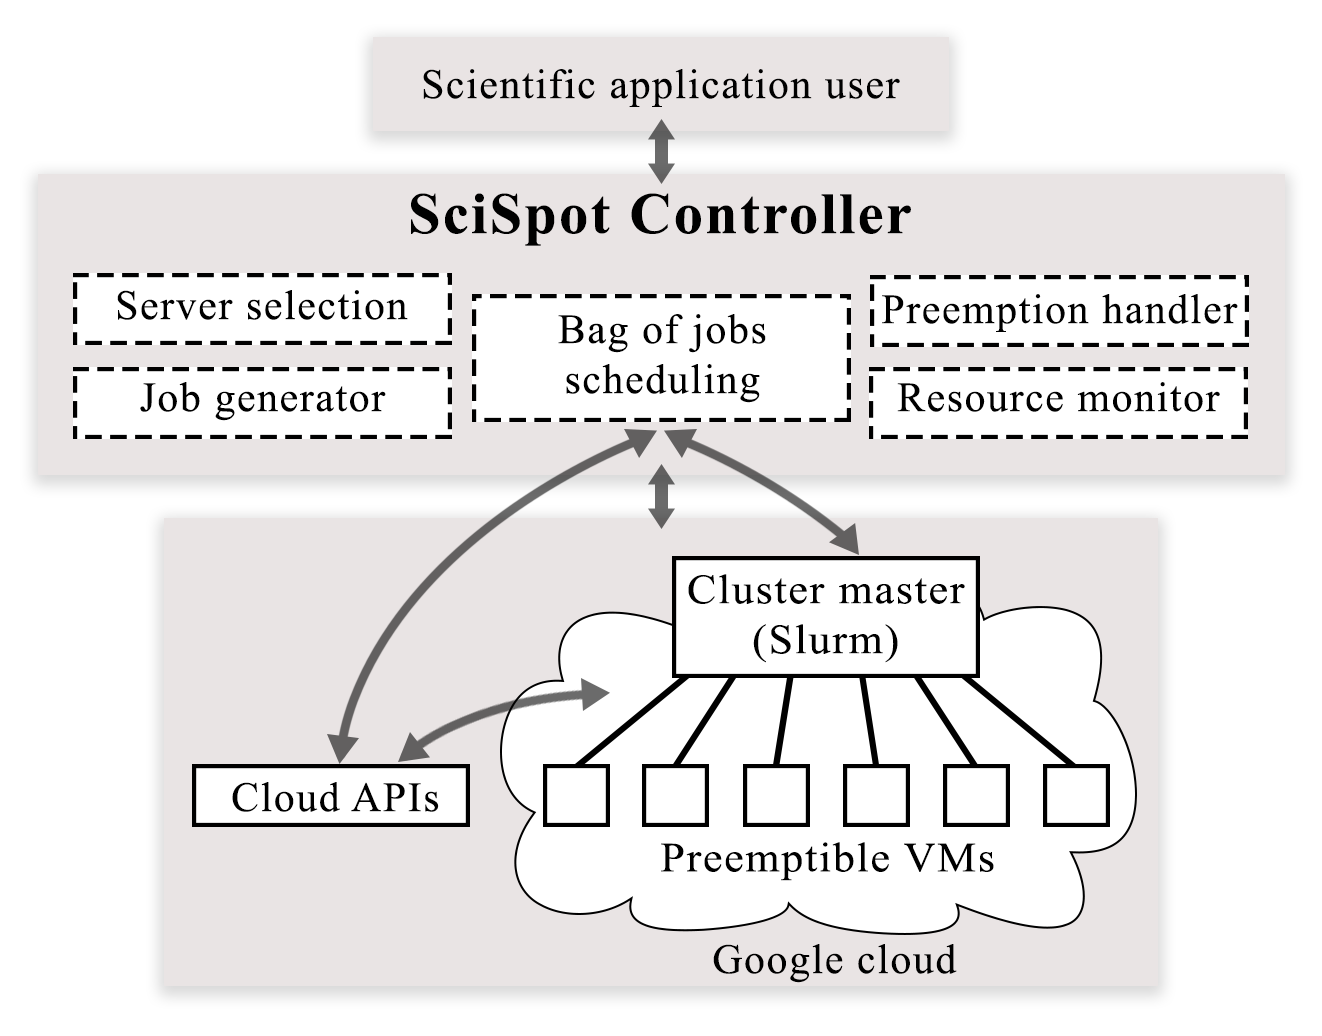
\includegraphics[width=0.3\textwidth]{../figures/Architecture.png}
\vspace*{\myfigspace}
  \caption{SciSpot architecture and system components.}
  \label{fig:arch}
  \vspace*{\myfigspace}
\end{figure}


\noindent \textbf{High-level workflow:} When a user wishes to run a bag of jobs, \sysname handles the provisioning of a cluster of transient cloud servers.
In addition, \sysname deals with the scheduling and monitoring of the bag of jobs, and with VM preemptions. 
Execution of a bag of jobs proceeds in two phases.
In the first phase, \sysname selects the ``right'' cluster configuration for a given application through a cost-minimizing exploration-based search policy, described in Section~\ref{subsec:server-selection}. 
In the second phase, \sysname proceeds to run the remaining jobs in the bag on the optimal cluster configuration. 

\prat{End design}


\sysname is implemented as a light-weight, extensible framework that makes it convenient and cheap to run scientific computing applications in the cloud.
We have implemented the \sysname prototype in Python in about 2,000 lines of code, and currently support running VMs on the Google Cloud Platform~\cite{gcp}. 
%
\sysname is implemented as a centralized controller, which implements the VM selection and job scheduling policies described in Section~\ref{sec:design}. 
The controller can run on any machine (including the user's local machine, or inside a cloud VM), and exposes an HTTP API to end-users. 
Users submit bags of jobs to the controller via the HTTP API, which then launches and maintains a cluster of cloud VMs, and maintains the job queue and metadata in a local database. 
To improve usability, we automatically generate parameter combinations for a given bag size, based on a user-provided json file with ranges and constraints for each parameter. 

\sysname integrates, and interfaces with two primary services.
First, it uses the Google cloud API~\cite{gcloud-api} for launching, terminating, and monitoring VMs.
Once a cluster is launched, it then configures a cluster manager such as Slurm~\cite{slurm} or Torque~\cite{torque}, to which it submits jobs. 
\sysname uses the Slurm cluster manager, with each VM acting as a Slurm ``cloud'' node, which allows Slurm to gracefully handle VM preemptions.
The Slurm master node runs on a small, 2 CPU non-preemptible VM, which is shared by all applications and users. 
\sysname monitors job completions and failures (due to VM preemptions) through the use of Slurm call-backs, which issue HTTP requests back to the \sysname controller.

%As part of \sysname, we also provide a base VM image with Slurm and MPI integration, along with commonly used libraries and benchmarks for scientific computing. To run an application, users must provide a location to the application source code or binaries. Integrating \sysname with container-based image management tools such as Docker~\cite{docker} and Singularity~\cite{kurtzer2017singularity} is part of our ongoing work. 





%%% Local Variables:
%%% mode: latex
%%% TeX-master: "paper"
%%% End:


%Opening is deliberately short because we gonna be running out of space

In this section, we present analytical and empirical evaluation of constrained preemptions.
We have already presented the statistical analysis of our model in Section~\ref{sec:failmodel}, and we now focus on answering the following questions: 

\begin{enumerate}
\item How do constrained preemptions impact the total running time of applications?

\item  What is the effect of our model-based policies when compared to existing transient computing approaches?

%\item What is the real-world cost and performance of running batch applications?

\item What is the cost and performance of our batch computing service for real-world workloads? 
  
\end{enumerate}




\noindent \textbf{Environment and Workloads:}
All our empirical evaluation is conducted on the Google Public cloud using our batch computing service described in the previous section. 
We use three scientific computing workloads that are representative of typical applications in the broad domains of physics, material sciences, and chemical engineering:

% open-source
%\vspace*{\tightext}
%\begin{description}
  %TODO: Need MAX two sentence descriptions

\noindent \textbf{Nanoconfinement.}
The nanoconfinement application launches molecular dynamics (MD) simulations of ions in nanoscale confinement created by material surfaces \cite{jyto,kadupitiya2017}.

\noindent \textbf{Shapes.} The Shapes application runs an MD-based optimization dynamics to predict the optimal shape of deformable, charged nanoparticles \cite{jto1,jjzo1}. 

\noindent \textbf{LULESH.} Livermore Unstructured Lagrangian Explicit Shock Hydrodynamics (LULESH)  is a popular benchmark for hydrodynamics simulations of continuum material models \cite{IPDPS13:LULESH,LULESH2:changes}. 
% \end{description}

% These examples are representative of typical scientific computing applications in the broad domain of physics, materials science, and chemical engineering. These three examples are implemented as parallel programs that use OpenMP and MPI parallel computing techniques. The first two are used in nanoscale materials research \cite{jso1,jso2,solis2013generating,jjzo1,jto1,jyto} and LULESH is a widely used benchmark \cite{IPDPS13:LULESH,LULESH2:changes}.

%All applications are run with default parameters unless otherwise stated.




\subsection{Impact of Constrained Preemptions on Job Running Times}

\begin{figure}[t]
  \subfloat[Computation wasted due to one preemption. \label{fig:vs-uniform}]
  {  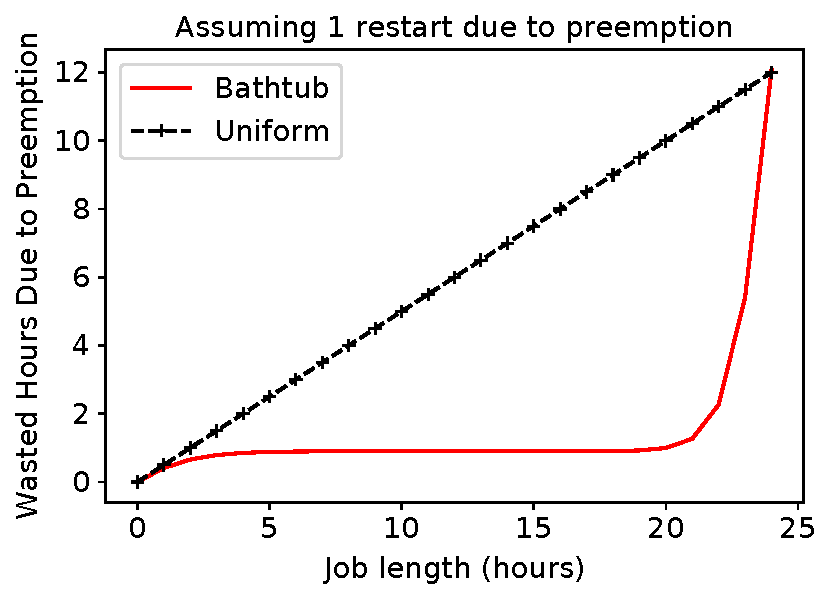
\includegraphics[width=0.3\textwidth]{../graphs/uniform-v-bathtub.pdf} }
  \\
    \subfloat[Expected increase in running time. \label{fig:vs-uniform-2}]
    {  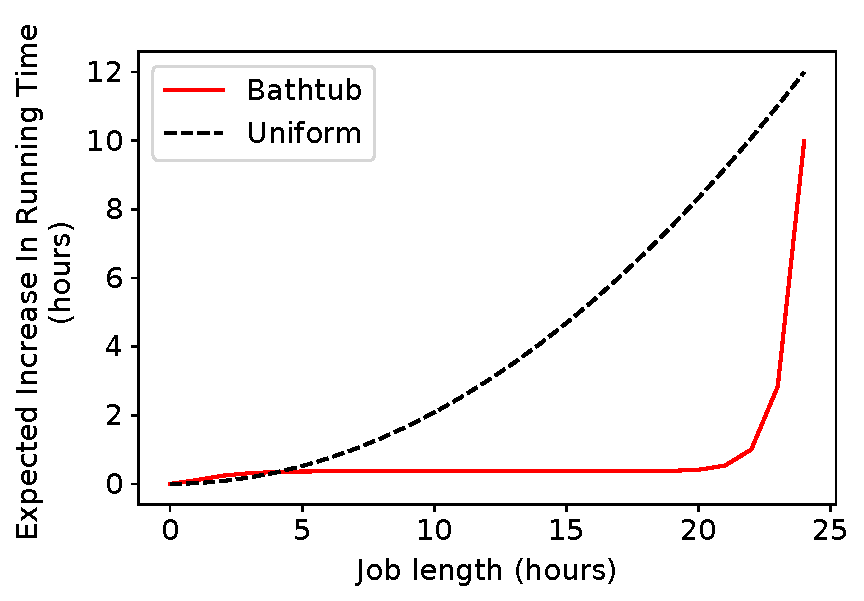
\includegraphics[width=0.3\textwidth]{../graphs/uniform-v-bathtub-2.pdf} }
    \caption{Wasted computation and expected increase in running time for uniform vs. baththub failures. For jobs $>5$ hours, bathtub distribution results in significantly lower wasted computation.}
  \label{fig:vs-uniform-both}
  
\end{figure}

%\caption{The expected wasted computation, given a single failure, is lower when preemptions are distributed in a bathtub shape, compared to uniformly distributed over the 24 hour interval}

We begin by examining how constrained preemptions impacts the total job running times. 
When a preemption occurs during the job's execution, it results in wasted work, assuming there is no checkpointing. 
This increases the job's total expected running time, since it must restart after a preemption.
In case of constrained preemptions, the expected waste depends both on the probability of job preemption, as well as \emph{when} the job was preempted. 


For a job of length $J$, the wasted work, assuming that the job faces a \emph{single} preemption, is $E[W_1(J)]$, and is given by Equation~\ref{eq:wasted}.
We first analyze this wasted work for jobs of different lengths in Figure~\ref{fig:vs-uniform}
We analyze two failure probability distributions for constrained preemptions: a uniform distribution such that $F(t) = 24-t$, and the bathtub shaped distribution with parameters corresponding to the \texttt{n1-highcpu-16} VM type shown in Figure~\ref{fig:gcp1}. 


For the uniform distribution, the wasted work is linear in the job length, and is given by $J/2$.
For the bathtub distribution, the wasted work is given by Equation~\ref{eq:wasted}, and is \emph{significantly} lower, especially for longer jobs (longer than 5 hours). 
With the bathtub distribution, jobs see a high rate of failure initially, but that also reduces the wasted work. 
Once jobs survive the initial high failure rate, the rate of failure is low, and thus the wasted work is more or less constant for all but the shortest and longest jobs. 



We now examine the expected increase in running time, that also accounts for the probability of failure, and is given by $P(\text{failure})*E[W_1]$. 
Figure~\ref{fig:vs-uniform-2} shows this expected increase in running times for jobs of different lengths.
We see that for uniformly distributed preemptions, the increase in running time is quadratic in the job length (and is given by $J^2/48$).
Interestingly, the high rate of early failures for the bathtub distribution results in a slightly worse (i.e., higher) running time for short jobs.
However for jobs longer than 5 hours, a cross-over point is reached, and the bathtub distribution provides a significantly lower overhead of preemptions. 
For instance, for a 10 hour job, the increase in running time is about 30 minutes, or 5\%. 
In contrast, if failures were uniformly distributed, the increase would be 2 hours. 


Thus, the bathtub preemptions are beneficial for applications and users, as the low failure rate during the middle periods results in significantly lower wasted work, compared to the uniformly distributed failures.
Since the failure rate distribution is ultimately controlled by the cloud provider, our analysis can be used to determine the appropriate distribution based on the job length distributions.
For instance, if short jobs are very common, then uniformly distributed preemptions are preferable, otherwise, bathtub distributions can offer significant benefits. 

\noindent \textbf{Result:} \emph{For constrained preemptions, bathtub distributions significantly reduce the expected increase in running times for medium to long running jobs, but are slightly inferior for short jobs.}




%%%%%%%%%%%%%%%%%%%%%%%%%%%%%%%%%%%%%%%%%%%%%%%%%%%%%%%%%%%%%%%%%%%%%%
\subsection{Model-based Policies}
\label{subsec:eval-policy}

We now evaluate the effectiveness of model-driven policies that we proposed earlier in Section~\ref{sec:policies}.
Specifically, we seek to compare the effectiveness of our job scheduling and checkpointing policies with existing transient computing approaches.



\subsubsection{Job Scheduling}

In the previous subsection, we have quantified the increase in running time due to preemptions, but we had assumed that jobs start on a newly launched server.
In many scenarios however, a server may be used for running a long-running sequence of jobs, such as in a batch-computing service. 
%
Our job scheduling policy is model-driven and decides whether to request a new VM for a job or run it on an existing VM.
A new VM may be preferable if the job starts running near the VM's 24 hour preemption deadline.
%However, since new VMs have a high initial rate of failure, we must be judicious 

Figure~\ref{fig:sched-bathtub} shows the effect of our job scheduling policy for a six hour job, for different job starting times (relative to the VM's starting time). 
We compare against a baseline of memoryless job scheduling that is not informed by constrained preemption dynamics.
Such memoryless policies are the default in existing transient computing systems such as SpotOn~\cite{spoton}. 
In the absence of insights about bathtub preemptions, the memoryless policy continues to run jobs on the existing VM. 
As the figure shows, the empirical job failure probability is bathtub shaped. 
However since the job is 8 hours long, with the memoryless policy, it will always fail when launched after $24-6=18$ hours.
In contrast, our model-based policy determines that after 18 hours, we will be better off running the job on a newer VM, and results in a much lower job failure probability (=0.4).
Thus, our model-based job scheduling policy can reduce job failure probability by taking into account the time-varying failure rates of VMs, which is not considered by existing systems that use memoryless scheduling policies.


\begin{figure}[t]
  \subfloat[Effect of job start time on the failure probability. \label{fig:sched-bathtub}]
  {  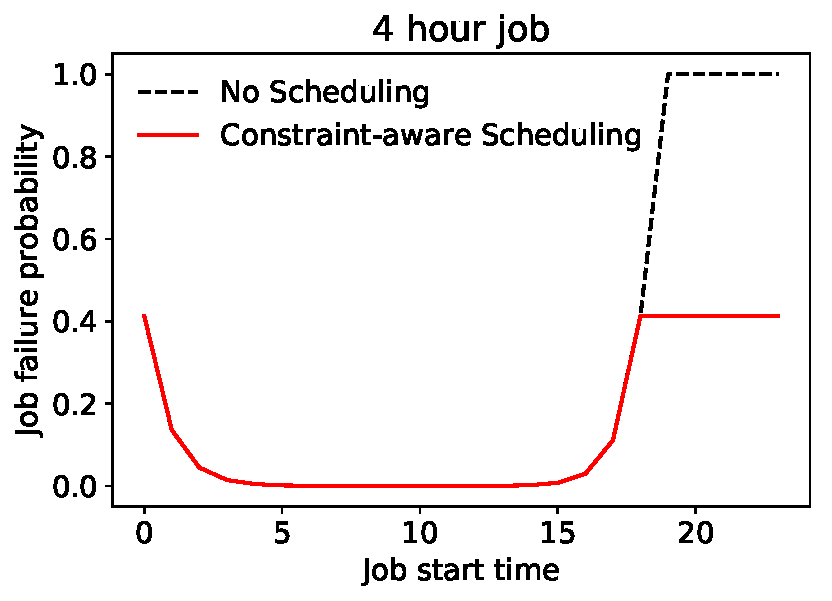
\includegraphics[width=0.35\textwidth]{../graphs/Sched-bathtub.pdf}}
  \\
  \subfloat[Job failure probability for jobs of different lengths. \label{fig:sched-all}]
  {  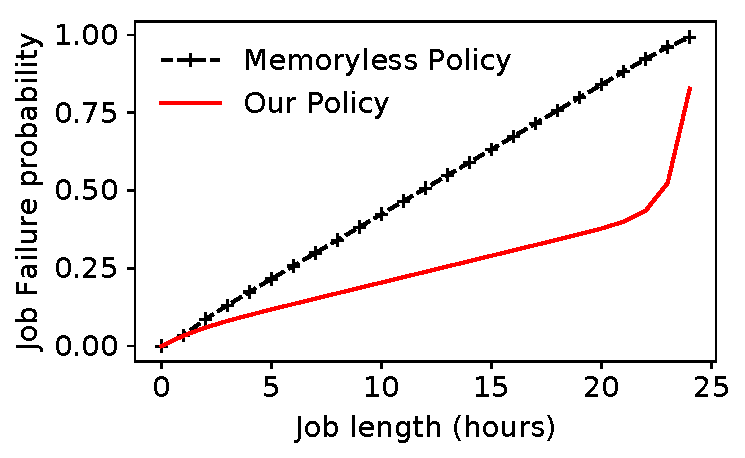
\includegraphics[width=0.35\textwidth]{../graphs/Sched-fail-prob.pdf}}
  \caption{Job failure probability is lower with our deadline aware policy across all job sizes.}
  \label{fig:sched-both}
\end{figure}

The job failure probability is determined by the job length and the job starting time.
We examine the failure probability for jobs of different lengths in Figure~\ref{fig:sched-all}, in which we average the failure probability across different start times.
We again see that our policy results in significantly lower failure probability compared to memoryless scheduling.
For all but the shortest and longest jobs, the failure probability with our policy is \emph{half} of that of existing memoryless policies.
This difference is primarily due to the differences in how the two policies perform for jobs launched near the end of the VM preemption deadline, which we examined previously in Figure~\ref{fig:sched-bathtub}. 


\noindent \textbf{Result:} \emph{Our model-based job scheduling and VM-reuse policy can decrease job failure probability by $2\times$.}



%%%%%%%%%%%%%%%%%%%%%%%%%%%%%%%%%%%%%%%%%%%%%%%%%%
\subsubsection{Checkpointing}
\label{subsec:eval-ckpt}

We now evaluate our model-based checkpointing policy, that uses a dynamic programming approach.
With our policy, the checkpointing rate is determined by the VM's current failure rate.
In contrast, all prior work in transient computing and most prior work in fault-tolerance assumes that failures are exponentially distributed (i.e., memoryless), and use the Young-Daly checkpointing interval.
In the Young-Daly approach, checkpoints are taken after a constant period given by $\tau \propto \sqrt{MTTF}$.
However in the case of constrained preemptions with bathtub distributions, the failure rate is time-dependent and not memoryless. 


The expected increase in running time for a 4 hour job is shown in Figure~\ref{fig:ckpt-4}, in which we account for both the increase due to the checkpointing overhead, as well as the expected recomputation due to preemptions. 
Throughout, we assume that each checkpoint takes 1 minute. 
The increase in running time depends on the failure rate and thus the job's starting time. 
With our model-based checkpointing policy, the increase in running time is bathtub shaped and is below 5\%, and around 1\% when the job is launched when the VM is between 5 and 15 hours old. 

We also compare with the Young-Daly periodic checkpointing policy, and use the initial failure rate of the VM to set the MTTF, which corresponds to an MTTF of 1 hour. 
This results in a high, constant rate of checkpointing, and thus increases the running time of the job by more than 25\%.
The increase in running time is primarily due to the overhead of checkpointing. 
Note that checkpointing with a lower frequency decreases the checkpointing overhead, but increases the recomputation required.

Next, we examine the expected running time of jobs of different length, when all jobs start at time=0, i.e, are launched on a freshly launched VM. 
Figure~\ref{fig:ckpt-start-0-relative} shows the expected increase in the running time of the jobs with our model-based checkpointing policy and the Young-Daly policy with MTTF=1 hour.
With our policy, the running times increase by 10\% for short jobs less than 2 hours long, and increase by less than 5\% for longer jobs.
In contrast, the Young-Daly policy yields a constant increase in running times of 25\%. 
Thus, our model-based policy is able to reduce the checkpointing overhead and thus reduce the performance overhead of running on preemptible VMs to below 5\%. 

\noindent \textbf{Result:} \emph{Our checkpointing policy can reduce the performance overhead of preemptions to under 5\%, which is $5\times$ better than conventional Young-Daly policies.}


\begin{figure}[t]
  \subfloat[Checkpointing overhead for different job starting times. \label{fig:ckpt-4}]
{  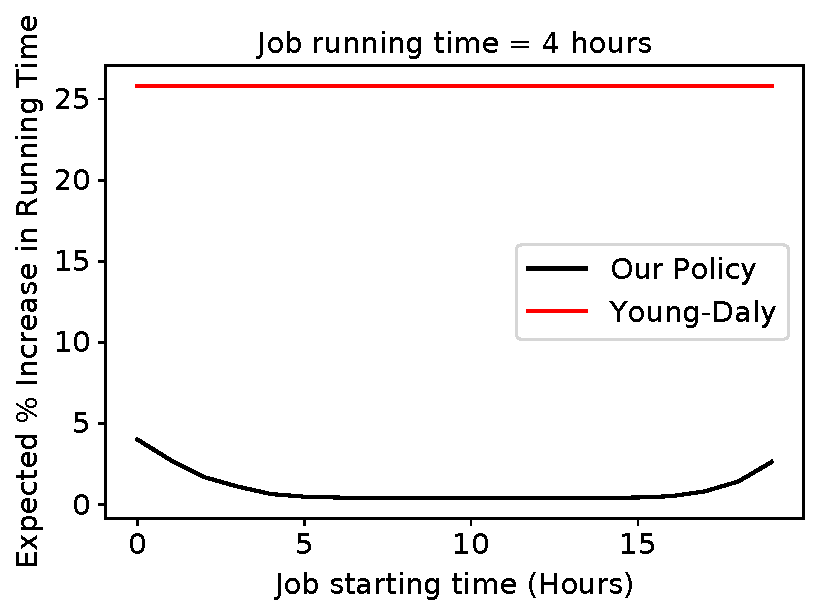
\includegraphics[width=0.35\textwidth]{../graphs/ckpt-4.pdf} }
%\hfill
% \subfloat[Running time with checkpointing when jobs start at time=0. \label{fig:ckpt-start-0}]
% {  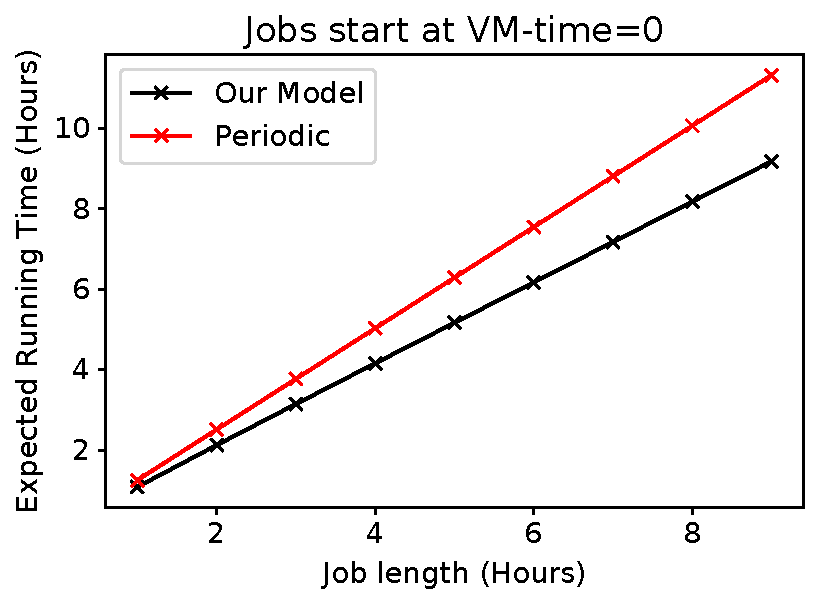
\includegraphics[width=0.3\textwidth]{../graphs/ckpt-start-0.pdf}}
% \hfill
\\
\subfloat[Increase in running time with checkpointing when jobs start at time=0. \label{fig:ckpt-start-0-relative}]
{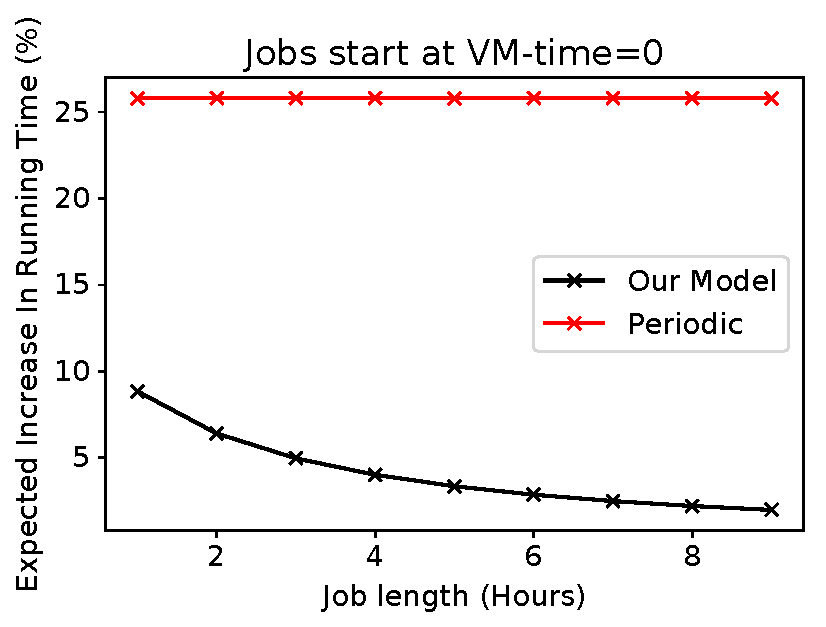
\includegraphics[width=0.35\textwidth]{../graphs/ckpt-start-relative.pdf}}

  \caption{Checkpointing effectiveness.}
  \label{fig:ckpt-all}
\end{figure}


%%%%%%%%%%%%%%%%%%%%%%%%%%%%%%%%%%%%%%%%%%%%%%%%%%

%\subsection{SciSpot Evaluation}
\subsection{Effectiveness on Scientific Computing Workloads}

We now show the effectiveness of our batch computing service on Google Preemptible VMs.
We run scientific simulation workloads described earlier in this section, and are interested in understanding the real-world effectiveness of our model-based service.
We use our model-driven job scheduling policy, but do not use checkpointing, since it requires additional 

%%%%%%%%%%%%%%%%%%%%%%%%%%%%%%%%%%%%%%%%%%%%%%%%%%


%As described in Section~\ref{sec:design}, applications can be deployed on multiple types of VMs in the cloud, with each VM type having a different ``size''.
%In our evaluation of parallel scientific computing applications that are CPU intensive, we are primarily interested in the number of CPUs in a VM.


%%%%%%%%%%%%%%%%%%%%%%%%%%%%%%%%%%%%%%%%%%%%%%%%%%


\begin{figure}[t]
  \centering
  \subfloat[Cost \label{fig:cost-only-bar}]
{  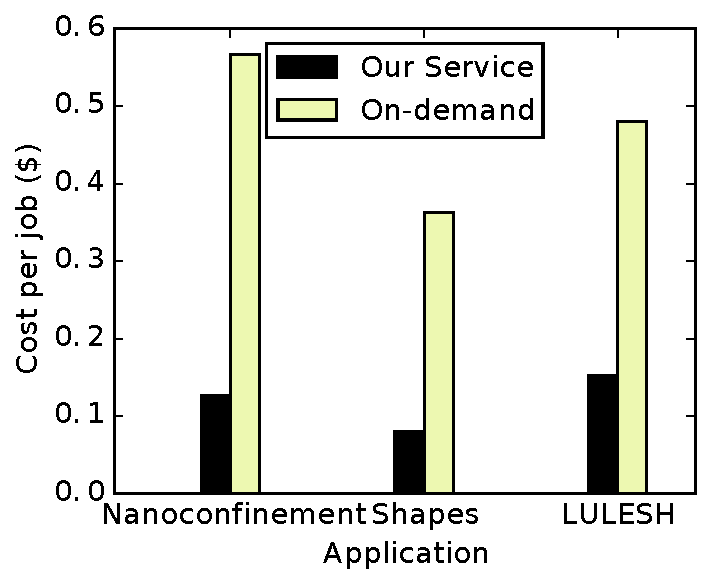
\includegraphics[width=0.25\textwidth]{../graphs/cost-vs-ondem.pdf} }
\hfill
\subfloat[Preemptions \label{fig:fails-time}]
{ 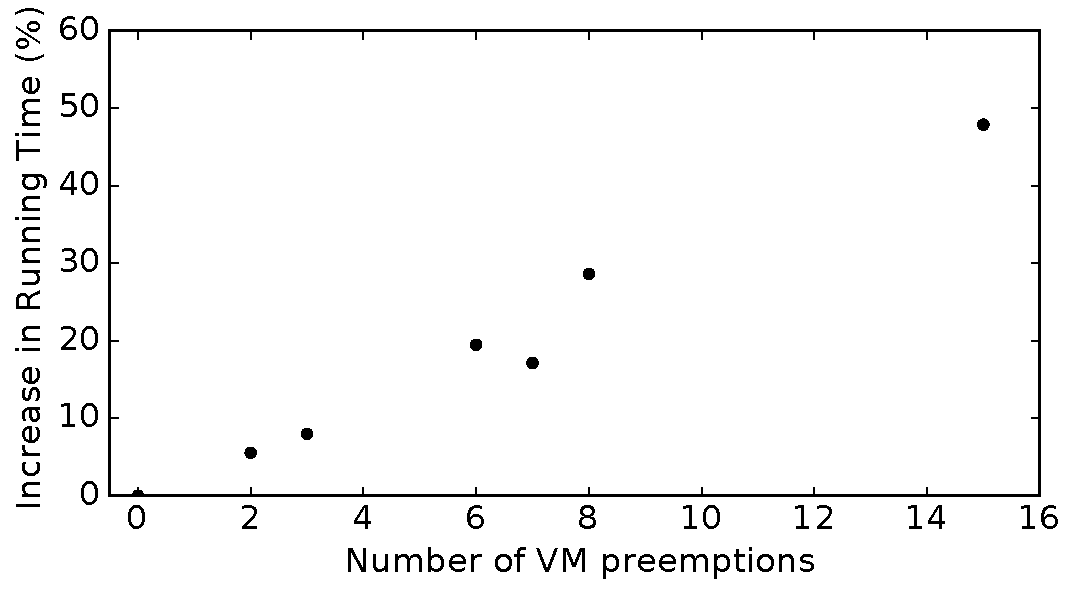
\includegraphics[width=0.2\textwidth]{../graphs/confin-fails-vs-time-relative.pdf} }
\label{fig:service-all}
\caption{Cost and preemptions with our service.}
\end{figure}  

%  \caption{SciSpot's use of preemptible VMs can reduce costs by up to $5\times$ compared to conventional cloud deployments, and 20\% compared to the state of the art EC2 spot instance selection (ExoSphere~\cite{exosphere}).}
%  \label{fig:cost-only-bar}
%    \vspace*{\myfigspace}


\noindent \textbf{Cost:}
The primary motivation for using preemptible VMs is their significantly lower cost compared to conventional ``on-demand'' cloud VMs that are non-preemptible.
To evaluate the cost of using our batch computing service, we run a bag of 100 jobs, all running on a cluster of 32 VMs of type \texttt{n1-highcpu-32}. 
Within a bag, different jobs are exploring different physical parameters, and job running times show little variance. 
Figure~\ref{fig:cost-only-bar} shows the cost of using Preemptible VMs compared to conventional on-demand VMs.
We see that for all the three applications, using our service can reduce costs by $5\times$.

We note that for this experiment, our  service was using model-driven job scheduling, but was not using checkpointing, since the applications lacked checkpointing mechanisms.
However, incorporating checkpointing would reduce the costs even further, since it would reduce the increase in running time (and server costs) due to recomputation.


\noindent \textbf{Preemptions:} 
Finally, we examine the effect of preemptions on the increase in running time under real-world settings.
We ran a cluster of 32 \texttt{n1-highcpu-32} VMs running the Nanoconfinement application, and repeated the experiment multiple times to observe the effect of preemptions.
Figure~\ref{fig:fails-time} shows the increase in running time of the entire bag of jobs, when different number of VM preemptions are observed during the entire course of execution.
We see that the net impact of preemptions results in a roughly linear increase in running time. 
Each preemption results in a roughly 3\% increase in running time, which validates our analytical evaluation shown earlier in Figure~\ref{fig:vs-uniform-2}.
The result also highlights the effectiveness of the job scheduling and VM-reuse policy, since most jobs run on the stable VMs, and  those that run on new VMs ``fail fast'' and result in only a small amount of wasted work and increase in running time. 


% \begin{figure}[t]
%   \centering 
%         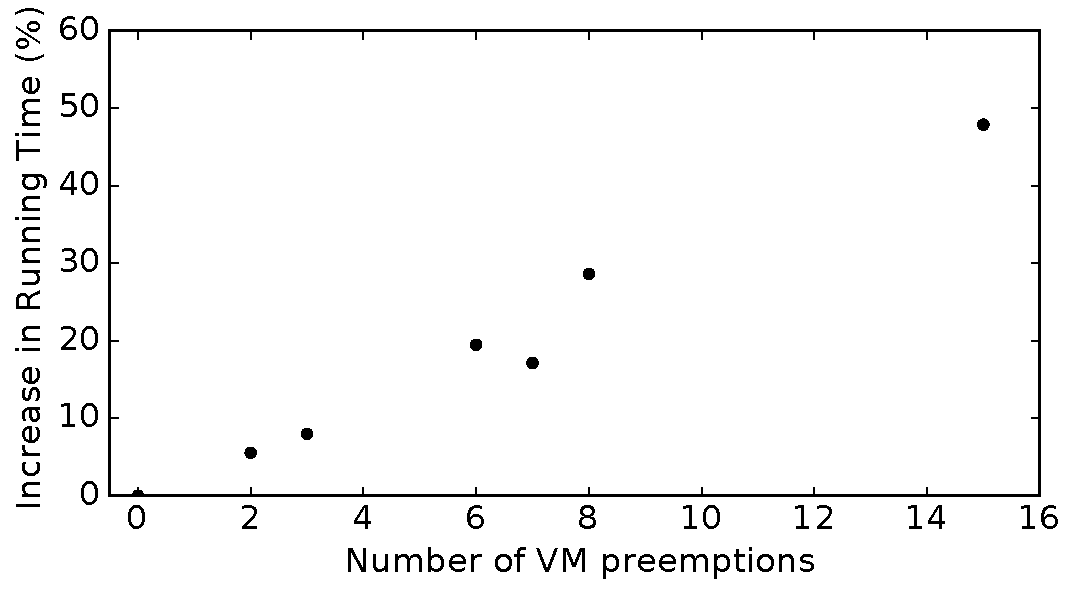
\includegraphics[width=0.22\textwidth]{../graphs/confin-fails-vs-time-relative.pdf}
%       \caption{The increase in running time due to preemptions is under 50\%, even at high preemption rates.}
%         %when the number of preemptions is high.}
%   \label{fig:fails-time}
% \end{figure}



\noindent \emph{\textbf{Result:} Our batch computing service can reduce costs by up to 5$\times$ compared to conventional on-demand cloud VMs. With the VM-reuse policy, the performance impact of preemptions is as low as 3\%.}
  %which is $20\times$ lower than a memoryless policy.}



%%%%%%%%%%%%%%%%%%%%%%%%%%%%%%%%%%%%%%%%%%%%%%%%%%
%HPC should be the last thing ?


% \begin{figure}
%   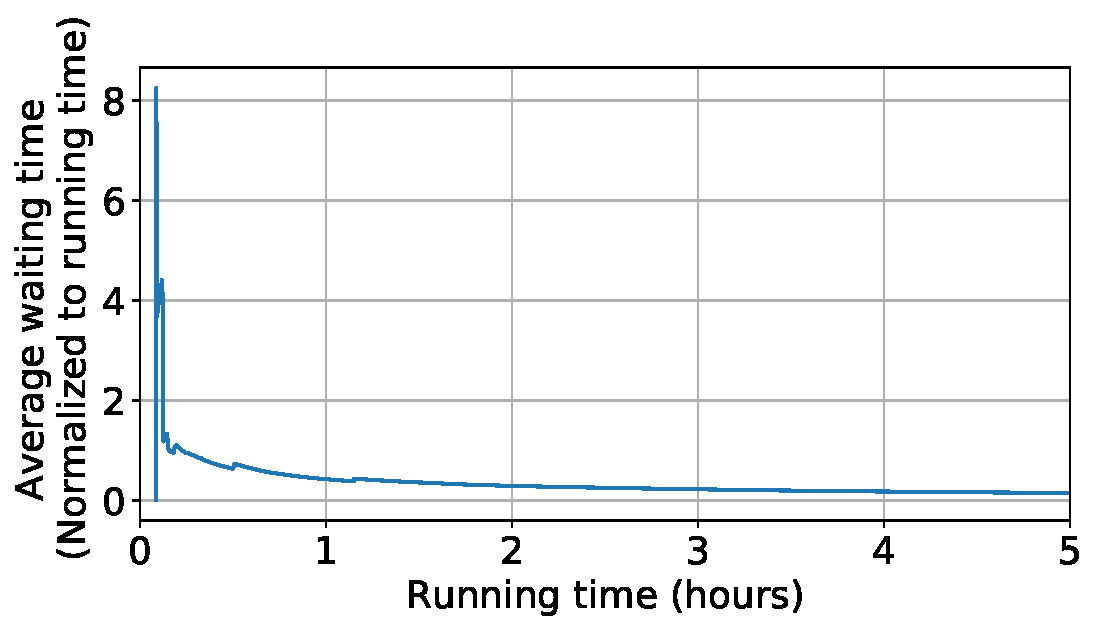
\includegraphics[width=0.4\textwidth]{../data/waiting_cumul.pdf}
%   \caption{The average waiting time (normalized to running time) of jobs of different length.}
%   \label{fig:hpc-wait-cdf}
% \end{figure}



%%% Local Variables:
%%% mode: latex
%%% TeX-master: "paper"
%%% End:
